\documentclass[conference]{IEEEtran}
\IEEEoverridecommandlockouts
\usepackage{amsmath,amssymb,amsfonts}
\usepackage{graphicx}
\usepackage{booktabs}
\usepackage{multirow}
\usepackage{xcolor}
\usepackage{tikz}
\usetikzlibrary{arrows.meta,positioning,fit,calc}
\usepackage{algorithm}
\usepackage{algpseudocode}
\usepackage{cite}
\usepackage[hidelinks]{hyperref}
\graphicspath{{../results/climate-rescue-2026-10-18/figures/}{../images/}}

\def\BibTeX{{\rm B\kern-.05em{\sc i\kern-.025em b}\kern-.08em
    T\kern-.1667em\lower.7ex\hbox{\sc e}\kern-.125em X}}

\begin{document}

\title{Vikasa: A Deterministic Individual-Based Simulator for Measuring the Critical Rate of Evolutionary Rescue Under Observed Climate Forcing}

\author{\IEEEauthorblockN{Sushanth Kasturi}
\IEEEauthorblockA{\textit{Vikasa Project} \\
Hyderabad, India}}

\maketitle

\begin{abstract}
Climate change threatens species not only through the magnitude of warming but
through its \emph{rate} relative to the speed at which populations can adapt.
Quantitative-genetic theory predicts a critical rate of environmental change above
which an evolving population can no longer track its moving optimum, yet this
threshold is rarely made concrete, reproducible and accessible to practitioners.
This paper presents \emph{Vikasa}, an open-source, deterministic, individual-based
eco-evolutionary simulator in which every animal inherits a six-gene body genome,
a behavioural temperament and a heritable thermal optimum, and chooses its own
actions through a transparent drive--utility arbiter. Temperature is forced by
NASA POWER monthly reanalysis records for real Indian regions combined with IPCC
AR6 shared socio-economic pathway (SSP) warming medians. A pre-registered rate
sweep of 216 simulations (9 warming rates $\times$ 2 inheritance arms $\times$ 12
seeds) measures a critical rate of $k_c=0.262\,^{\circ}$C per generation (95\%
CI 0.234--0.291) with heritable tolerance against $0.067\,^{\circ}$C per
generation (0.052--0.080) for a zero-heritability control, a paired rescue gain of
$+0.196\,^{\circ}$C per generation. Adaptation lag grows linearly with the rate
($r=0.85$), matching the Lynch--Lande prediction. Translating $k_c$ through SSP
warming rates yields a critical generation time of about 6.4 years under SSP5-8.5,
verified by direct simulation. A Sobol analysis on a Gaussian-process surrogate
shows that seasonal amplitude relative to tolerance breadth dominates survival.
The measured results are wrapped in two decision-support tools, a Species Risk
Checker and a Conservation Planner, and a GPU-instanced 3D client that renders the
full population at 60 frames per second on integrated graphics. Three of eight
pre-registered criteria failed and are reported as findings.
\end{abstract}

\begin{IEEEkeywords}
artificial life, individual-based model, evolutionary rescue, climate change,
thermal tolerance, sensitivity analysis, Gaussian process, reproducible simulation,
conservation decision support
\end{IEEEkeywords}

\section{Introduction}
Whether a species survives climate change depends on two clocks: how fast its
environment changes and how fast it can evolve. Populations that breed quickly
accumulate many generations of selection per degree of warming, whereas
long-lived species experience the same warming in only a handful of generations.
Theory formalises this as \emph{evolutionary rescue}: a population that would
otherwise decline can be saved by adaptive genetic change if that change is
fast enough \cite{gomulkiewicz1995,bell2009}. Quantitative-genetic models of a
moving phenotypic optimum predict a \emph{critical rate} of environmental change
\cite{lynch1993,burger1995,chevin2010}. Below it, the mean phenotype settles at a
constant lag behind the optimum; above it, the lag grows without bound and the
population goes extinct.

Analytical results of this kind rest on idealised assumptions: infinite or large
populations, Gaussian fitness surfaces, constant genetic variance and no
behaviour. Real populations are finite, structured by age, limited by food and
subject to demographic chance. Individual-based models (IBMs) relax these
assumptions by simulating each organism explicitly \cite{deangelis2014,grimm2006},
but IBM results are frequently hard to reproduce, hard to inspect and disconnected
from observed climate data.

This paper describes \emph{Vikasa} (Sanskrit for ``development'' or ``evolution''),
a deterministic artificial-life laboratory built to close that gap. Its
contributions are:
\begin{enumerate}
\item A fully seeded, invariant-audited IBM in which inherited body traits,
temperament and a heritable thermal optimum interact with foraging, mating, care,
conflict, starvation and age-dependent mortality (Section~\ref{sec:model}).
\item A climate twin driven by NASA POWER reanalysis and IPCC AR6 pathways, with
an asymmetric thermal-performance curve and heat-induced sterility
(Section~\ref{sec:climate}).
\item A pre-registered measurement of the critical warming rate with and without
heritability, a global Sobol sensitivity analysis and a Gaussian-process (GP)
surrogate, including the criteria that failed (Sections~\ref{sec:protocol}--\ref{sec:results}).
\item A translation of the measured threshold into a \emph{critical generation
time} per emission pathway, checked by direct simulation of real regions.
\item Two practitioner tools, the Species Risk Checker and the Conservation
Planner, plus a real-time 3D client that renders the authoritative engine state
without influencing it (Section~\ref{sec:tools}).
\end{enumerate}

The climate data are real, but the organism is a generic model, not a calibrated
species. All numbers below should be read as properties of this model.

\section{Related Work}
Artificial-life systems such as Tierra \cite{ray1991}, Avida \cite{ofria2004} and
PolyWorld \cite{yaeger1994} demonstrated open-ended evolution of digital organisms
but were not designed to answer ecological questions with external forcing.
Ecological IBMs \cite{deangelis2014} are commonly documented using the ODD
(Overview, Design concepts, Details) protocol \cite{grimm2006,grimm2020}, which
Vikasa adopts for its climate module.

Evolutionary rescue has been studied analytically \cite{gomulkiewicz1995,lynch1993,burger1995},
experimentally in microbes \cite{bell2009}, and in reviews of adaptation to
climate change \cite{hoffmann2011}. Chevin \emph{et al.} \cite{chevin2010} added
plasticity to the moving-optimum model. Thermal-performance curves that fall off
faster on the warm side are well established for ectotherms
\cite{huey1989,deutsch2008}, and fertility often fails at temperatures below the
lethal limit \cite{walsh2019}. Janzen's climatic-variability hypothesis
\cite{janzen1967} motivates scaling tolerance breadth with local seasonality.

For uncertainty quantification, Vikasa uses variance-based Sobol indices
\cite{sobol2001} estimated with Saltelli sampling and Jansen estimators
\cite{saltelli2010,jansen1999}, Latin hypercube designs \cite{mckay1979} and GP
regression \cite{rasmussen2006}. Proportions are reported with Wilson score
intervals \cite{wilson1927}. Evolutionary change is decomposed with Price's
equation \cite{price1970,frank2012}. On the management side, assisted gene flow
\cite{aitken2013} and assisted colonisation \cite{hoegh2008} are the interventions
that the Conservation Planner sizes. To our knowledge no existing open tool couples
a reproducible eco-evolutionary IBM, observed climate records and these
management outputs in one auditable pipeline.

\section{System Architecture}
\label{sec:arch}
Vikasa separates simulation from presentation (Fig.~\ref{fig:arch}). A Python
\texttt{SimulationEngine} owns all persistent state and advances fixed discrete
\emph{ticks}. Clients---a headless experiment runner, a Pygame 2D laboratory, the
Godot~4 \emph{Living Biome} and three browser applications---only observe the engine
or issue explicit commands; none decide outcomes. Rendering may lag or disconnect
without altering the simulation.

\begin{figure}[t]
\centering
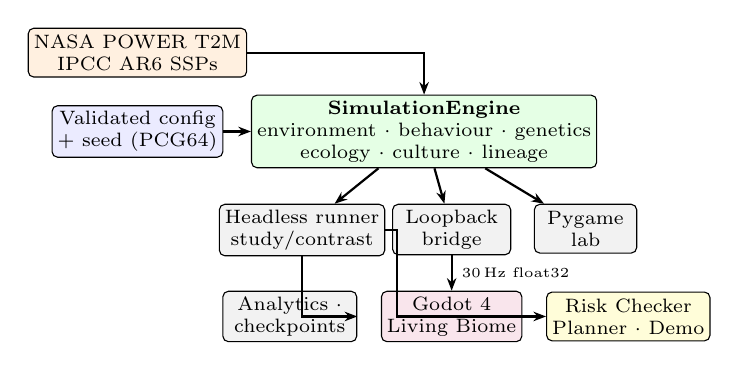
\begin{tikzpicture}[
  box/.style={draw, rounded corners=2pt, align=center, font=\scriptsize, minimum height=0.62cm, inner sep=2pt},
  arr/.style={-{Stealth[length=1.6mm]}, thick}]
\node[box, fill=blue!8, minimum width=2.1cm] (cfg) {Validated config\\+ seed (PCG64)};
\node[box, fill=green!10, right=0.35cm of cfg, minimum width=3.3cm] (eng) {\textbf{SimulationEngine}\\environment $\cdot$ behaviour $\cdot$ genetics\\ecology $\cdot$ culture $\cdot$ lineage};
\node[box, fill=orange!12, above=0.35cm of cfg, minimum width=2.1cm] (data) {NASA POWER T2M\\IPCC AR6 SSPs};
\node[box, fill=gray!10, below=0.45cm of eng, xshift=-1.55cm, minimum width=1.6cm] (head) {Headless runner\\study/contrast};
\node[box, fill=gray!10, below=0.45cm of eng, xshift=0.35cm, minimum width=1.5cm] (bridge) {Loopback\\bridge};
\node[box, fill=gray!10, below=0.45cm of eng, xshift=2.05cm, minimum width=1.3cm] (pg) {Pygame\\lab};
\node[box, fill=purple!10, below=0.45cm of bridge, minimum width=1.6cm] (godot) {Godot 4\\Living Biome};
\node[box, fill=gray!10, left=0.3cm of godot, minimum width=1.7cm] (ana) {Analytics $\cdot$\\checkpoints};
\node[box, fill=yellow!15, right=0.3cm of godot, minimum width=1.7cm] (tools) {Risk Checker\\Planner $\cdot$ Demo};
\draw[arr] (cfg) -- (eng);
\draw[arr] (data) -| (eng.north);
\draw[arr] (eng) -- (head);
\draw[arr] (eng) -- (bridge);
\draw[arr] (eng) -- (pg);
\draw[arr] (bridge) -- node[right, font=\tiny]{30\,Hz float32} (godot);
\draw[arr] (head) |- (ana);
\draw[arr] (head.east) -- ++(0.15,0) |- (tools.west);
\end{tikzpicture}
\caption{Vikasa architecture. The engine is the single source of truth; every
client consumes immutable snapshots or issues explicit, logged commands.}
\label{fig:arch}
\end{figure}

\subsection{Deterministic tick schedule}
One NumPy PCG64 generator owns every stochastic outcome. Stable integer IDs order
all order-sensitive updates and break ties. Algorithm~\ref{alg:tick} lists the
schedule. Above 40 animals, cognition is staggered deterministically by
$(\text{tick}+\text{id}) \bmod 6$, while movement and vital processes run every
tick; contest opportunities are sampled every four ticks. These schedules apply
identically to GUI and headless runs, so a seed reproduces the same world on the
same software and numerical platform.

\begin{algorithm}[t]
\caption{One engine tick}
\label{alg:tick}
\small
\begin{algorithmic}[1]
\State update seasons, climate temperature and active events
\State step plant/water field (spatial profile only)
\State erode food under weather; regenerate food patches
\State build spatial hash; perceive; decide (staggered); move; pay energy
\If{$\text{tick} \bmod 4 = 0$} resolve contests \EndIf
\State resolve feeding contention by squared distance, then ID
\State resolve mutual mate choice and births (Price observer)
\State apply starvation, injury, senescence and age-ceiling deaths
\State $\text{tick} \gets \text{tick}+1$; update culture and satisfaction
\State sample metrics every \texttt{sample\_interval} ticks
\end{algorithmic}
\end{algorithm}

\subsection{Persistence, provenance and audit}
Checkpoint format version~3 serialises the RNG state, entities, behavioural state,
lineage, environment, culture and the fractional food-spawn accumulator, so a
saved run continues bit-for-bit. Saving writes a flushed temporary file and
atomically replaces the destination; versions 1 and 2 migrate in memory.
Invariant checks (for example, founders $+$ births $-$ deaths $=$ living) run
throughout. Evidence packages carry configuration and source hashes and a SHA-256
manifest, and the study runner rejects publication if source files change mid-run.

\subsection{Real-time presentation}
The bridge serves three loopback channels: a length-prefixed little-endian float32
push stream at up to 30\,Hz (a 24-value header and 18 values per animal: position,
velocity, energy, action, three genes, temperament, flags, dynasty, generation,
age, injury), a slim JSON explanation document at 2.5\,Hz that carries full detail
only for the watched animal, and a sequenced event feed so no birth, death or clash
is lost between polls. The Godot client bakes one procedural quadruped mesh and
animates gait and gene-driven morphology in a vertex shader, so the whole
population costs two instanced draw calls. On an Intel Iris Xe laptop this raised
the frame rate from 13--35 to a locked 59--60 frames per second and cut draw calls
from about 2{,}300 to about 20 for the 3D world.

\begin{figure}[t]
\centering
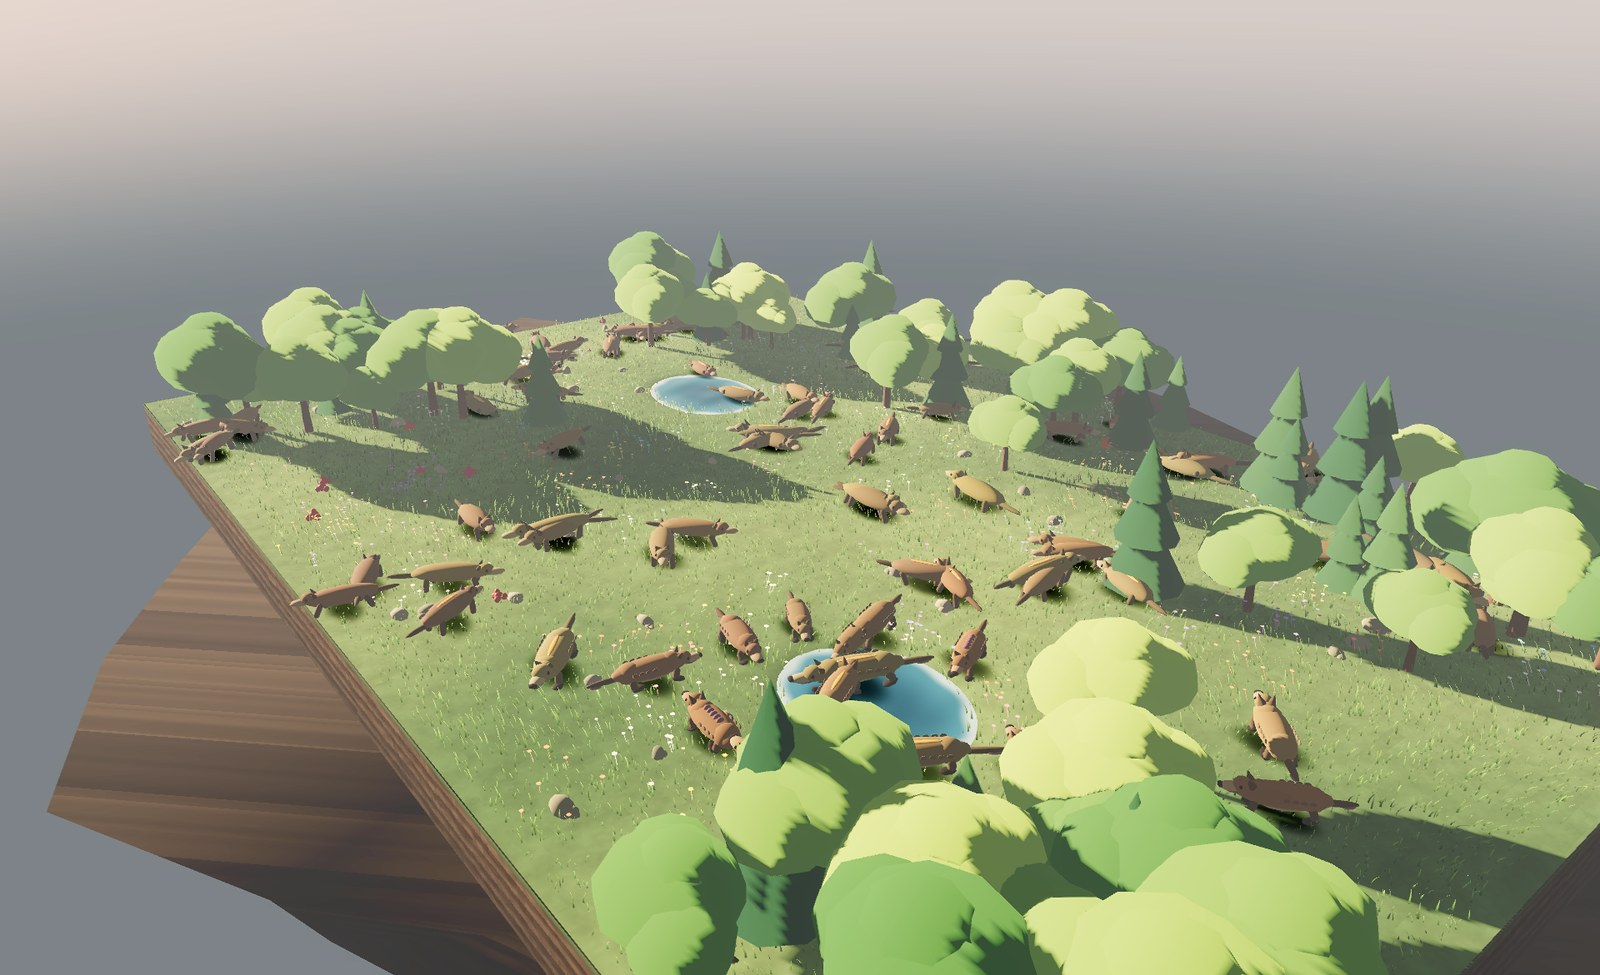
\includegraphics[width=\columnwidth]{showcase-hero.jpg}
\caption{The Godot~4 Living Biome client rendering a seeded engine state. Every
animal, birth, death and clash comes from the Python engine; terrain, daylight and
water are presentation only.}
\label{fig:hero}
\end{figure}

\section{Organism and Ecology Model}
\label{sec:model}
\subsection{Genome and inheritance}
Each animal carries an ordered body genome
$\mathbf{g}=(\text{size},\text{speed},\text{perception},\text{metabolism},\text{threshold},\text{fertility})$,
each gene bounded on $[L_i,H_i]$. Founders draw $g_i\sim U(L_i,H_i)$. Arithmetic
crossover sets $c_i=\alpha_i a_i+(1-\alpha_i)b_i$ with $\alpha_i\sim U(0,1)$;
each gene then mutates with probability $p_m$ by
$\varepsilon_i\sim\mathcal{N}(0,\sigma(H_i-L_i))$ and is clamped. The showcase uses
$p_m=0.1$ and $\sigma=0.075$. Aggression, resilience and sociability form a
separately inherited temperament in $[0,1]$. An opt-in diploid profile maps two
phased binary haplotypes through dominance-weighted dosages
$\delta_\ell=(h^{(1)}_\ell+h^{(2)}_\ell)/2+d_\ell|h^{(1)}_\ell-h^{(2)}_\ell|/2$
and normalised effect matrices onto the six traits, with per-interval
recombination during meiosis.

\subsection{Energy and mortality}
Basal expenditure per tick is
\begin{equation}
C_b=c_b\,\frac{1+s/8}{m}\;\mu_{\text{event}}\,\mu_{\text{season}}\,\mu_{\text{injury}}\,\mu_{\text{health}}\,(1+1.5\,\varsigma),
\end{equation}
where $s$ is size, $m$ metabolism and $\varsigma$ thermal stress
(Section~\ref{sec:climate}); movement costs
$c_m\,d\,(0.5+s/8)(0.5+v/4)\,\mu_{\text{weather}}$ for distance $d$ and speed $v$.
Energy at or below zero increments a starvation counter that decays when energy
recovers; death occurs after 12 accumulated ticks, so starvation is delayed and
reversible. Age-dependent mortality follows a Gompertz hazard
\begin{equation}
\mu(a)=\mu_0\,e^{\,b\max(0,a-a_0)},\qquad P(\text{death})=1-e^{-\mu(a)},
\end{equation}
with $\mu_0=2\times10^{-5}$, $b=0.002$ and $a_0=1800$ ticks in the showcase and a
12{,}000-tick hard ceiling. This replaced a fixed 1{,}100-tick lifespan that, with
same-aged founders, caused a founder die-off and extinction by tick 3{,}000; the
old configuration is retained as a control.

\subsection{Drives, utilities and arbitration}
Six normalised drives are recomputed from reserves, injury and local perception:
survival, foraging, mating, offspring care, danger avoidance and territory. For
example, with $E/E_{\max}$ the reserve fraction and $I$ injury,
$\text{survival}=\mathrm{clip}(0.65(1-E/E_{\max})+0.35I)$. Eight candidate
actions (explore, forage, rest, seek mate, care, flee, patrol, challenge) are
scored as
\begin{equation}
U_a=\mathrm{clip}\Big(\sum_k A_{a,k}\,D_k+R_a-T_a-X_a-K_a\Big),
\end{equation}
a weighted drive affinity plus an action-specific reward minus travel, exposure and
conflict costs. Unavailable actions are excluded. Danger at or above 0.75 forces
flight; survival pressure at or above 0.65 forces foraging; injury at or above 0.65
forces rest. Otherwise the current action is kept if it is within a hysteresis
margin of 0.08 of the best, and remaining near-ties are broken by a seeded softmax,
$P(a)\propto\exp((U_a-U_{\max})/\tau)$ with $\tau=0.08$. Every animal exposes its
action, its reason and its utility breakdown, so behaviour is inspectable rather
than opaque.

\subsection{Reproduction, conflict and culture}
Mating requires mutual choice, minimum age, an energy threshold, an off-cooldown
state and headroom under the population cap; each parent contributes half the
newborn's energy. Fertility shortens cooldown as
$\max(1,\mathrm{round}(c(1-0.5f)))$. Contests are rare: encounter risk is capped
at 0.09 and gated by close range plus hunger or an explicit challenge, and fatal
risk is bounded by 0.42. Repeated shared cues (season turns, drought, heat,
storms, victories) can found named traditions that spread through contact; this is
a rule-based transmission mechanism, not a model of language or religion.

\subsection{Evolutionary observers}
Two observers quantify change without consuming simulation randomness. At every
birth event, an exact Price decomposition \cite{price1970,frank2012} is computed
over the \emph{entire} pre-birth living population. With trait $z_i$, offspring
contribution $w_i$ (0.5 per child per parent, zero for non-parents) and weighted
descendant mean $z'_i$,
\begin{equation}
\Delta\bar z=\underbrace{\frac{\mathrm{Cov}(w,z)}{\bar w}}_{\text{selection}}
+\underbrace{\frac{\overline{w(z'-z)}}{\bar w}}_{\text{transmission}},
\end{equation}
which holds to floating-point rounding; for $z=(1,3)$, $w=(1,3)$, $z'=(2,4)$ it
gives selection 0.5, transmission 1.0 and total 1.5. This is an accounting
identity, not a causal estimate. At export, traits are normalised to their
configured span, $x_{ij}=(z_{ij}-a_j)/(b_j-a_j)$, and the sample covariance, its
eigen-decomposition and the participation ratio
$D_{\text{eff}}=1/\sum_k f_k^2$ (with $f_k$ the variance fraction of component
$k$) summarise how many directions of trait variation are effectively present.
Generation depth is one plus the deepest parent's depth, traversed iteratively
with cycle detection.

\begin{table}[t]
\caption{Principal parameters of the two main worlds}
\label{tab:params}
\centering
\setlength{\tabcolsep}{3pt}
\begin{tabular}{lcc}
\toprule
Parameter & Showcase & Climate rescue\\
\midrule
World (units) & $720\times480$ & $480\times320$\\
Founders / population cap & 64 / 180 & --- / 70\\
Size, speed bounds & [2.5, 8], [0.5, 4] & [2.5, 8], [0.5, 4]\\
Perception bounds & [25, 150] & [20, 80]\\
Mutation $p_m$, $\sigma$ & 0.1, 0.075 & 0.1, 0.075\\
Initial / max energy & 125 / 230 & 125 / 230\\
Basal, movement cost & 0.09, 0.026 & 0.09, 0.026\\
Min. age, cooldown (ticks) & 90, 100 & 40, 40\\
Mate radius, offspring energy & 90, 60 & 80, 60\\
Food spawn rate, patch energy & 0.9, 30 & 0.45, 30\\
Mortality & Gompertz & as configured\\
Tolerance $\omega$, warm ratio & --- & 4\,$^{\circ}$C, 0.6\\
Segregation / mutation SD & --- & 0.4 / 0.1\,$^{\circ}$C\\
\bottomrule
\end{tabular}
\end{table}

\subsection{Weather and spatial ecology}
Seasons advance every 96 ticks and modulate food productivity
($1.12, 0.96, 0.84, 0.72$) and metabolic demand. Scheduled events (drought, heat,
cold, storm, flood, wildfire, disease, abundance) compose additively into a health
pressure $H$ and a food-decay rate; exposure injury per tick is
$0.018\,H(1-0.75\rho)(1+0.6h)$ for resilience $\rho$ and hunger $h$. An optional
$24\times16$ spatial profile adds a plant-energy field with exact logistic growth,
water-limited transpiration and a conservative five-point transport step
$X'=(1-4d)X+d\sum_{\text{nbr}}X$ with $0\le d\le1/4$; audited ledgers verify that
initial stock plus growth minus losses minus harvest equals the current stock.

\section{Climate Forcing and Thermal Tolerance}
\label{sec:climate}
\subsection{Observed data and pathways}
Temperature is $T(t)=T_{\text{clim}}(\text{month}(t))+\Delta(\text{year}(t))$.
The climatology is the 1991--2020 monthly mean of NASA POWER 2\,m air temperature
derived from MERRA-2 reanalysis \cite{gelaro2017}, retrieved for 1981--2025 and
stored with request URL, retrieval time and the SHA-256 of the raw response. The
anomaly $\Delta$ is linear from 2005 (the centre of the AR6 1995--2014 reference
period) to 2090, reaching the IPCC AR6 WG1 Table~4.5 global medians
\cite{ipcc2021}: 0.9, 1.8, 2.8 and 3.5\,$^{\circ}$C for SSP1-2.6, SSP2-4.5,
SSP3-7.0 and SSP5-8.5, optionally scaled by a regional factor. Twenty-four Indian
sites spanning Kochi to Leh are bundled, and any coordinate can be fetched.

\subsection{Thermal performance and its costs}
Each animal carries a thermal optimum $\theta$. With mismatch $\Delta T=T-\theta$
and breadth $\omega$, stress is one minus an asymmetric Gaussian performance
curve \cite{huey1989},
\begin{equation}
\varsigma=1-\exp\!\left(-\frac{\Delta T^2}{2w^2}\right),\quad
w=\begin{cases}0.6\,\omega,&\Delta T>0\\ \omega,&\Delta T\le0,\end{cases}
\label{eq:stress}
\end{equation}
so the warm side falls off faster. Stress multiplies basal cost by $1+1.5\varsigma$,
adds injury $0.02(\varsigma-0.3)/0.7$ per tick when $\varsigma>0.3$, and blocks
breeding while $\varsigma>0.7$, representing heat-induced sterility \cite{walsh2019}.

\subsection{Inheritance arms}
In the \emph{heritable} arm, offspring follow the infinitesimal model
$\theta_{\text{child}}=\bar\theta_{\text{parents}}+\mathcal{N}(0,0.4)+\mathcal{N}(0,0.1)$
($^{\circ}$C; segregation plus mutation). In the \emph{control} arm, offspring draw
$\theta$ afresh from the founder distribution $\mathcal{N}(\bar T+\Delta_0,1)$:
identical standing variation but zero heritability. Any difference between arms is
therefore attributable to inheritance.

\section{Experimental Protocol and Statistics}
\label{sec:protocol}
\subsection{Generation calibration and rescue phases}
Ticks have no intrinsic real-time meaning, so results are expressed per generation.
The generation interval $G$ is measured as the reciprocal slope of mean living
ancestral depth against tick, at zero warming, averaged over three seeds; the
$480\times320$ rescue world gives $G=469$ ticks. Each run has 5 generations of
burn-in, 20 generations of warming at rate $r$ ($^{\circ}$C per generation) and
5 generations of hold, with one climate year per generation, Western Ghats
climatology and $\omega=4\,^{\circ}$C. Outcomes are survival, extinction
generation, population before warming, at minimum and at the end, the evolved
shift in mean $\theta$, the adaptation lag over the last five warming generations,
and the rescue signature (a dip below 50\% followed by recovery to $\ge80\%$).

\subsection{Statistical design}
\textbf{Rate sweep.} Nine rates from 0 to 0.4 $\times$ two arms $\times$ 12 seeds
(216 runs). Survival per cell uses Wilson 95\% intervals. A lightly penalised
logistic regression (L2, $C=10$ on the scaled rate, which stays finite under
perfect separation) gives $\mathrm{logit}\,p=\beta_0+\beta_1 r$, and the
critical rate is $k_c=-\beta_0/\beta_1$ at $p=0.5$, with a 2{,}000-resample
bootstrap CI. The rescue gain uses a paired bootstrap over seeds.

\textbf{Sensitivity.} Six inputs (warming rate, tolerance breadth 2--8\,$^{\circ}$C,
seasonal amplitude 0.5--8\,$^{\circ}$C, standing SD 0.25--2\,$^{\circ}$C,
segregation SD 0--1\,$^{\circ}$C and carrying-capacity scale 0.5--1.5) were
sampled with two 192-run Latin hypercubes (384 runs) plus 48 held-out runs. A GP
with a Mat\'ern-5/2 kernel plus white noise regresses the final-to-pre-warming
population ratio; survival probability is $P(\text{ratio}>\tau)$ under the
predictive normal, with $\tau$ learned as the midpoint between the largest extinct
and smallest surviving ratio. First- and total-order Sobol indices are estimated on
the surrogate with Saltelli sampling ($n=4{,}096$) and Jansen estimators:
\begin{equation}
S_i=\frac{V-\tfrac12\mathbb{E}[(f_B-f_{AB_i})^2]}{V},\;
S_{T,i}=\frac{\tfrac12\mathbb{E}[(f_A-f_{AB_i})^2]}{V}.
\end{equation}

\textbf{Regional assessment.} Three regions $\times$ four SSPs $\times$ 12 seeds,
for a reference organism ($\omega=4\,^{\circ}$C) and a locally adapted organism
($\omega=1.5\times$ seasonal amplitude), run on the real monthly cycle from 2025.

\textbf{Pre-registration.} Eight success criteria were fixed in a plan document
before the production run, and no parameter was changed afterwards.

\section{Results}
\label{sec:results}
\subsection{Evolution quadruples the survivable warming rate}
Table~\ref{tab:kc} and Fig.~\ref{fig:surv} summarise the sweep. Heritable
populations survived every seed up to $0.15\,^{\circ}$C per generation, 9/12 at
0.2, 3/12 at 0.3 and none at 0.4. Controls began failing at 0.075 and none survived
0.1. Inheritance raises the survivable rate by a factor of about four.

\begin{table}[t]
\caption{Critical warming rate (full profile, 12 seeds per cell)}
\label{tab:kc}
\centering
\begin{tabular}{lcc}
\toprule
Arm & $k_c$ ($^{\circ}$C/gen) & 95\% CI\\
\midrule
Heritable thermal tolerance & \textbf{0.262} & 0.234--0.291\\
Control (no heritability) & 0.067 & 0.052--0.080\\
Rescue gain (paired bootstrap) & \textbf{+0.196} & 0.165--0.230\\
\bottomrule
\end{tabular}
\end{table}

\begin{figure}[t]
\centering
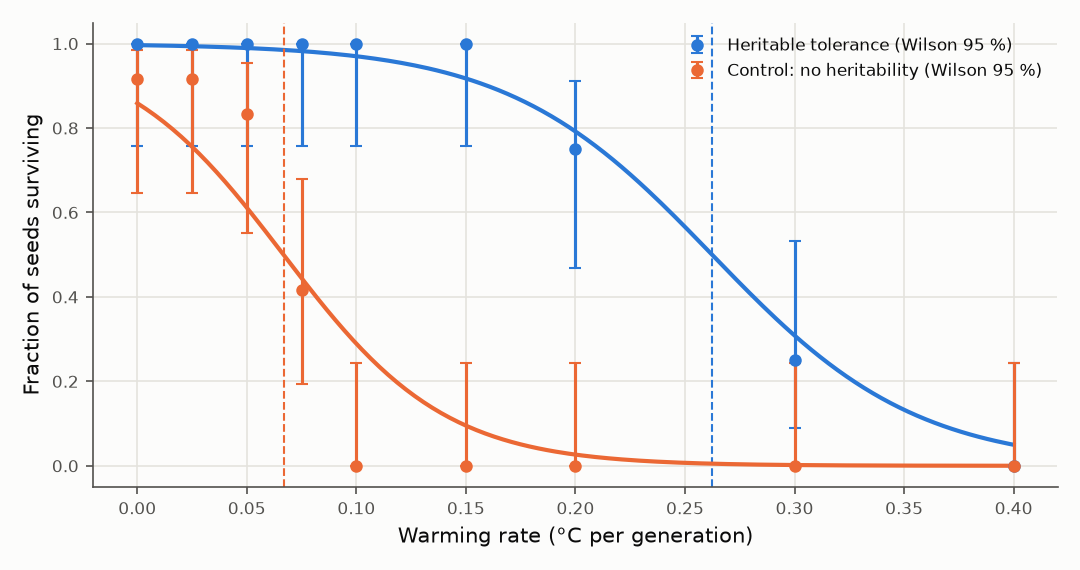
\includegraphics[width=\columnwidth]{survival_curve.png}
\caption{Survival probability against warming rate for heritable and control arms,
with Wilson 95\% intervals per cell and fitted logistic curves.}
\label{fig:surv}
\end{figure}

\subsection{Adaptation tracks warming with a growing lag}
The evolved shift in mean optimum grew with the rate: $+1.2$, $+2.9$ and
$+4.5\,^{\circ}$C at 0.1, 0.2 and 0.3\,$^{\circ}$C per generation, against 2, 4
and 6\,$^{\circ}$C of total warming. The lag behind the moving optimum rose linearly
with a slope of 6.4\,$^{\circ}$C per ($^{\circ}$C/generation), Pearson $r=0.85$ over
$n=81$ surviving runs (Fig.~\ref{fig:lag}), as the Lynch--Lande model predicts.
Near $k_c$, 17--25\% of surviving runs showed the classic rescue signature of a dip
below half size followed by recovery (Fig.~\ref{fig:traj}).

\begin{figure}[t]
\centering
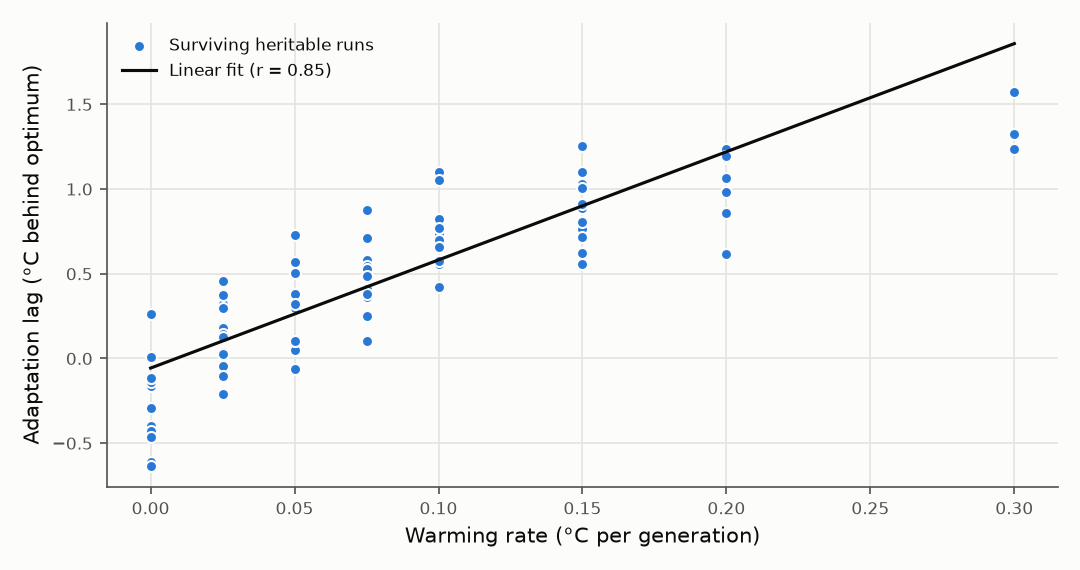
\includegraphics[width=\columnwidth]{lag_vs_rate.png}
\caption{Adaptation lag over the final five warming generations versus warming
rate for surviving heritable runs.}
\label{fig:lag}
\end{figure}

\begin{figure*}[t]
\centering
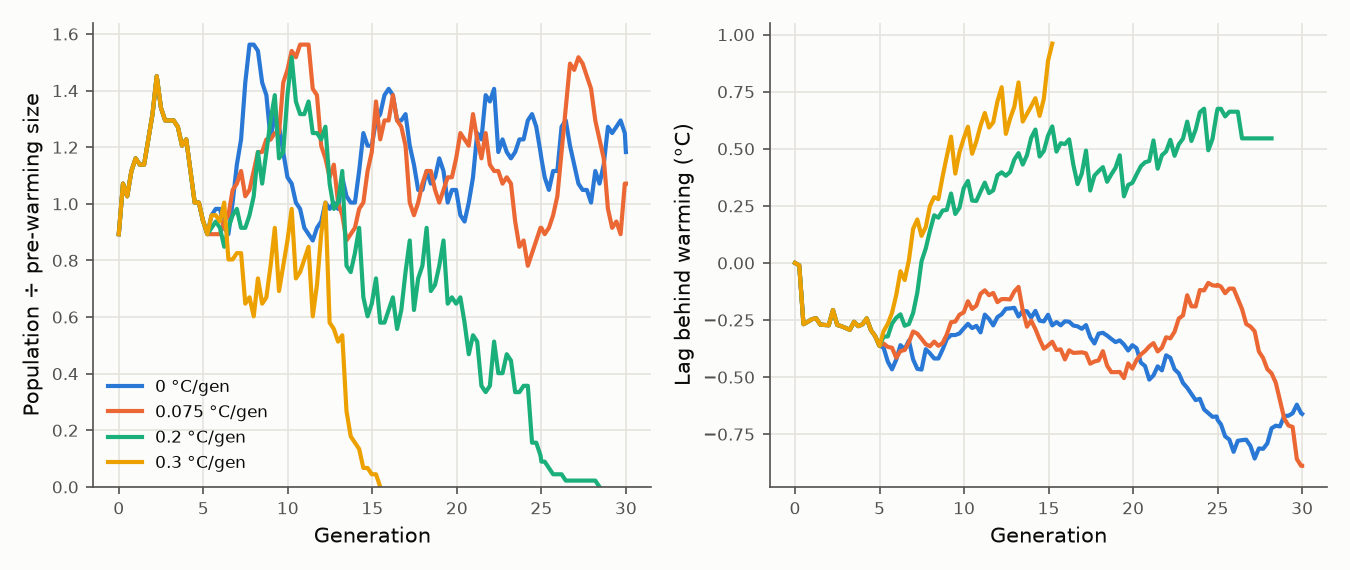
\includegraphics[width=0.88\textwidth]{trajectories.png}
\caption{Population and lag trajectories across the burn-in, warming and hold
phases. Near the critical rate some populations dip below half size and recover:
the signature of evolutionary rescue.}
\label{fig:traj}
\end{figure*}

\subsection{What decides survival}
Total-order Sobol indices (Fig.~\ref{fig:sobol}) were: seasonal amplitude 0.66,
tolerance breadth 0.30, warming rate 0.22, segregation SD 0.20, carrying capacity
0.13 and standing variation $\approx0$. Seasonal swings relative to tolerance
breadth dominate because many combinations in the explored ranges are lethal before
any warming starts. These indices are conditional on the explored ranges.
The surrogate reached a hold-out AUC of 0.93 for survival but an $R^2$ of only 0.51
on the population ratio (Fig.~\ref{fig:parity}); because the Sobol indices are
computed on the surrogate's survival probability, their ranking is more reliable
than their exact magnitudes.

\begin{figure}[t]
\centering
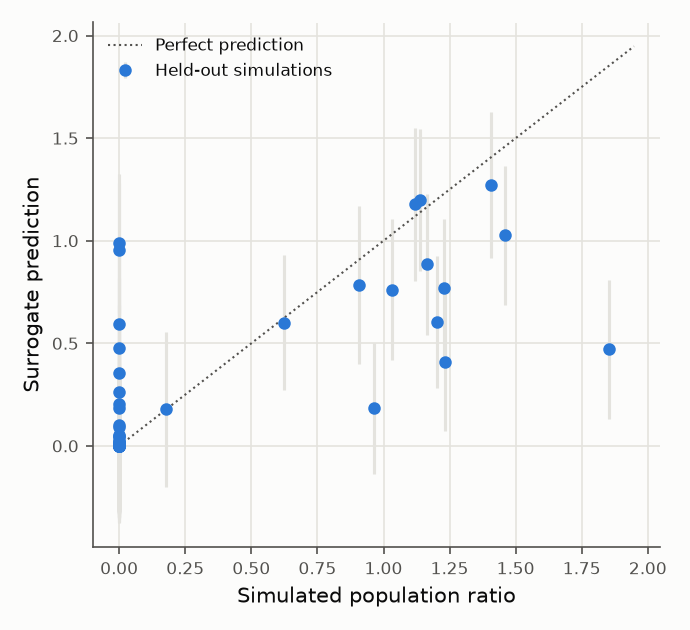
\includegraphics[width=0.78\columnwidth]{surrogate_parity.png}
\caption{GP surrogate parity on held-out design points: predicted versus simulated
final-to-pre-warming population ratio.}
\label{fig:parity}
\end{figure}

\begin{figure}[t]
\centering
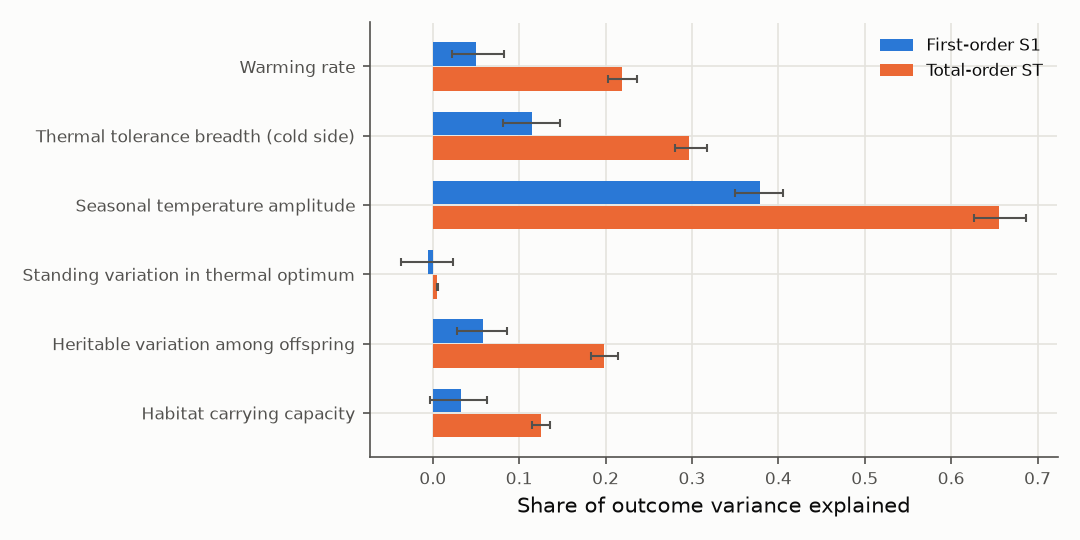
\includegraphics[width=\columnwidth]{sobol_bars.png}
\caption{First-order ($S_1$) and total-order ($S_T$) Sobol indices of survival
probability, with bootstrap intervals, estimated on the GP surrogate.}
\label{fig:sobol}
\end{figure}

\subsection{Real regions and the critical generation time}
For an organism with a one-year generation time, regional warming of
0.011--0.041\,$^{\circ}$C per generation is far below $k_c$, and every viable
population persisted ($p\ge0.92$, $n=12$, all SSPs, 2025--2065). Viability today,
however, depends on seasonality: the reference organism ($\omega=4\,^{\circ}$C) is
not viable under Delhi NCR's $\pm11.1\,^{\circ}$C or the Sundarbans'
$\pm5.4\,^{\circ}$C cycles even without warming, whereas locally adapted
organisms with breadth $1.5\times$ amplitude persist under every SSP.

Dividing $k_c$ by each pathway's warming rate yields the critical generation time
(Table~\ref{tab:gen}): species whose generations are longer fall behind. Direct
simulation of the Western Ghats on the real monthly cycle confirms the threshold
for six-year species, whose survival falls to 0.50 (95\% CI 0.25--0.75) under
SSP5-8.5, where warming per generation (0.247) is approximately $k_c$
(Table~\ref{tab:direct}). For twelve-year species, 2025--2100 spans only about six
generations, so less warming accumulates and survival exceeds the first-order rule;
the rule is therefore conservative for long-lived species over this century.

\begin{table}[t]
\caption{Critical generation time $k_c/\dot T$ by emission pathway}
\label{tab:gen}
\centering
\begin{tabular}{lcc}
\toprule
Scenario & $\dot T$ ($^{\circ}$C/yr) & Critical generation time (yr)\\
\midrule
SSP1-2.6 & 0.011 & 24.8 (22.1--27.5)\\
SSP2-4.5 & 0.021 & 12.4 (11.0--13.7)\\
SSP3-7.0 & 0.033 & 8.0 (7.1--8.8)\\
SSP5-8.5 & 0.041 & \textbf{6.4} (5.7--7.1)\\
\bottomrule
\end{tabular}
\end{table}

\begin{table}[t]
\caption{Direct check, Western Ghats, 2025--2100, 12 seeds each}
\label{tab:direct}
\centering
\setlength{\tabcolsep}{4pt}
\begin{tabular}{lcccl}
\toprule
Gen. & SSP & $^{\circ}$C/gen & Survival (95\% CI) & Verdict\\
\midrule
6 yr & 2-4.5 & 0.127 & 1.00 (0.76--1.00) & persists\\
6 yr & 3-7.0 & 0.198 & 0.67 (0.39--0.86) & at risk\\
6 yr & 5-8.5 & 0.247 & 0.50 (0.25--0.75) & at risk\\
12 yr & 2-4.5 & 0.254 & 0.92 (0.65--0.99) & persists\\
12 yr & 3-7.0 & 0.395 & 0.50 (0.25--0.75) & at risk\\
12 yr & 5-8.5 & 0.494 & 0.25 (0.09--0.53) & at risk\\
\bottomrule
\end{tabular}
\end{table}

\subsection{Pre-registered criteria}
Table~\ref{tab:crit} reports all eight criteria. C4 failed instructively: within
each generation heat kills cold-adapted individuals, so the \emph{surviving}
control population's mean optimum moves by about half as much as the heritable
arm's even though nothing is inherited. Viability selection within a generation
thus mimics part of an evolutionary response in cross-sectional means. S9 failed
because single-run outcomes are partly chance: even a perfect predictor explains at
most about 78\% of single-run variance in the sweep. S10 failed because seasonal
amplitude and breadth outrank the warming rate over the explored ranges.

\begin{table}[t]
\caption{Criteria fixed before the production run}
\label{tab:crit}
\centering
\setlength{\tabcolsep}{3pt}
\begin{tabular}{llp{3.6cm}}
\toprule
ID & Result & Criterion and measured value\\
\midrule
C1 & PASS & Persist without warming: 12/12\\
C2 & PASS & Faster warming lowers survival: $\rho=-0.84$\\
C3 & PASS & Heritability raises $k_c$: gain CI 0.165--0.230\\
C4 & FAIL & Optima track $\ge50\%$ of warming \emph{and} $\ge2\times$ control shift\\
C5 & PASS & Lag grows with rate: $r=0.85$\\
C6 & PASS & No invariant violations or failed runs: 0/0\\
S9 & FAIL & Surrogate hold-out $R^2\ge0.7$, AUC $\ge0.85$: got 0.51, 0.93\\
S10 & FAIL & Rate in top two drivers: ranks third ($S_T=0.22$)\\
\bottomrule
\end{tabular}
\end{table}

\subsection{Ecological baselines}
Independently of climate, the showcase world (64 founders, $720\times480$, cap 180)
was run for 12{,}000 ticks on seeds 2026, 7 and 41. All three persisted with
123, 117 and 114 living animals, 799, 720 and 717 births and deepest living
ancestral generations of 23, 23 and 20, with zero invariant failures (Wilson
survival interval $[0.44,1.00]$), whereas the preserved extinction-control
configuration went extinct at ticks 2{,}870, 2{,}589 and 2{,}265. In a seed-blocked
800-tick weather laboratory, baseline worlds ended with 160--175 animals, drought
with 22--24, and a severe storm bundle caused extinction at ticks 348--370;
the mean population change relative to the matched baseline was $-46.0$ (paired
bootstrap $[-49.2,-40.8]$) for drought and $-88.5$ ($[-94.8,-81.1]$) for storm.

\section{Decision-Support Tools}
\label{sec:tools}
\subsection{Species Risk Checker}
A user picks a place, a generation time (3 months to 50 years) and a tolerance
mode (specialist, local or generalist: $1\times$, $1.5\times$ or $2.5\times$ the
local seasonal swing) and an SSP. Step one is a seasonal screen: founders start at
the local annual mean and Eq.~(\ref{eq:stress}) is applied to the hottest and
coldest months; peak stress above 0.75 is \emph{not viable}, 0.65--0.75
\emph{borderline} and below 0.65 \emph{viable}. With no fitted parameters, this
screen reproduces all five published baseline verdicts of the regional assessment,
a property enforced by a unit test (Table~\ref{tab:screen}). Step two converts warming per generation into
survival with and without evolution through the measured logistic curve. Inputs
more than 25\% outside the measured domain are labelled \emph{indicative}, and a
live check (2 calibration seeds, 4 rescue seeds, Wilson intervals) is offered as
the authority when the two disagree.

\begin{table}[t]
\caption{Parameter-free seasonal screen versus published verdicts}
\label{tab:screen}
\centering
\setlength{\tabcolsep}{4pt}
\begin{tabular}{lccll}
\toprule
Assessment & $\omega$ ($^{\circ}$C) & Peak $\varsigma$ & Screen & Published\\
\midrule
W. Ghats, reference & 4.0 & 0.53 & viable & viable\\
Sundarbans, reference & 4.0 & 0.78 & not viable & not viable\\
Sundarbans, local & 8.2 & 0.30 & viable & viable\\
Delhi NCR, reference & 4.0 & 1.00 & not viable & not viable\\
Delhi NCR, local & 16.6 & 0.42 & viable & viable\\
\bottomrule
\end{tabular}
\end{table}

For example, a six-year species of local tolerance in Hyderabad
(annual mean 26.0\,$^{\circ}$C, seasons $\pm6.4\,^{\circ}$C, $\omega=9.6\,^{\circ}$C)
is viable today with a peak hot-season stress of 0.55, faces
$0.247\,^{\circ}$C of warming per generation under SSP5-8.5 (94\% of $k_c$), and
receives an instant estimate of 58\% survival with evolution versus 1\% without.
Because the reference curve was measured for a narrower 4\,$^{\circ}$C organism,
the estimate is flagged as indicative; the live check for this broader-tolerance
organism returned 4 of 4 survivors, and the application shows both and states
which to trust.

\subsection{Conservation Planner}
For a watchlist, the planner runs a first-order adaptation-lag model per species
for every year 2025--2100. The optimum follows warming at up to
$k_c/G_{\text{yr}}$\,$^{\circ}$C per year; breeding fails in the first year that
worst-month stress exceeds 0.75. Assisted gene flow is sized by grid search and
18-step bisection for the smallest optimum shift that keeps the species breeding to
2100, rounded up so the reported shift never falls short. Refuges are sites of the
same habitat class that stay below the failure line every year 2030--2100, with
translocated stock conservatively not credited with local adaptation. Priority is
\begin{equation}
P=100\left[0.55\,(1-p_{\text{surv}})+0.45\,\frac{2100-y_{\text{fail}}}{75}\right],
\end{equation}
set to 100 if not viable today and to at least 70 if breeding fails by 2050, with
tiers Critical ($\ge70$), High ($\ge45$), Watch ($\ge20$) and Low. On an
illustrative 14-species Indian watchlist, the planner ranks the Asian elephant in
Bengaluru first (score 80; breeding fails 2059 with evolution, 2046 without;
$+1.27\,^{\circ}$C gene flow; refuge Munnar, 326\,km) and the olive ridley in
Chennai second (69; fails 2077 versus 2054; $+0.66\,^{\circ}$C; refuge Kochi,
559\,km). Where the measured survival curve and the place-specific timeline
disagree, it places ``confirm with the live simulation'' first rather than hiding
the conflict. Outputs are a script-free HTML report, CSV and JSON.

\section{Discussion}
\subsection{Interpretation}
The measured threshold has a simple practical reading: under high emissions,
generic organisms in this model whose generations exceed about six years are at
real risk, and about 25 years under SSP1-2.6. Emission pathways therefore matter
most for long-lived species, and the Planner makes this explicit through its
pathway table. The Sobol result adds a caution that is easy to miss when focusing on
warming rates: present-day seasonality relative to tolerance breadth can make a
place unlivable before any warming occurs, which is why the screen is applied first.

\subsection{Reproducibility as a design principle}
Every claim in this paper is regenerated by a single resumable command
(\texttt{vikasa climate pipeline --profile full}). Extinct and failed runs are
retained rather than dropped, uncertainty is reported with intervals rather than
point values, and the three failed criteria are published unchanged. The codebase
comprises about 12{,}100 lines of Python, 5{,}700 lines of GDScript and shader
code, and 554 automated tests including a regression that locks the seasonal
screen to the published verdicts.

\subsection{Software verification}
The test suite spans every layer: hand-derived checks of logistic plant growth,
diffusion conservation and positivity; exact Price identities and negative chart
axes; Gompertz hazard behaviour and repeatable mortality; checkpoint round-trips
and strict rejection of corrupted budgets or non-integer identifiers; deterministic
replay of identical seeds; the bridge's binary frame contract; the climate data
parser, SSP anomaly, logistic fit, Wilson interval and Sobol estimators (validated
on the Ishigami function); and the planner's bisection, refuge search and report
rendering. Headless Godot scripts smoke-test the scene contract, behaviour
presentation, chart rendering and the narrated demo autopilot. A separate
benchmark tool compares a historical spatial index against the current one while
requiring identical full checkpoint digests at warm-up and final boundaries; it
measured a 14--20\% throughput gain with no change to biology.

\subsection{Limitations}
The organism is generic; only the climate forcing is observed data. There is no
phenotypic plasticity, behavioural thermoregulation, dispersal or food web, so
temperature acts only through the tolerance curve, and real species with
shade-seeking behaviour will usually fare better than these verdicts suggest.
Populations are small (tens of animals), so demographic stochasticity is stronger
than in most wild populations. Regional warming is the global-mean AR6 pathway
times a regional factor rather than a downscaled projection, and reanalysis grid
cells smooth mountains and coasts. Generation times in the example watchlist are
illustrative orders of magnitude. The engine is two-dimensional; terrain, daylight
and weather particles in the 3D client are scenery that does not feed back into
the model.

\section{Conclusion and Future Work}
Vikasa turns the abstract critical rate of evolutionary rescue into a measured,
reproducible and usable quantity. In a deterministic individual-based world forced
by observed temperatures, heritable thermal tolerance raises the survivable warming
rate from 0.067 to 0.262\,$^{\circ}$C per generation, the adaptation lag grows
linearly as theory predicts, and the result translates into a critical generation
time of about six years under SSP5-8.5. Wrapping these measurements in a risk
checker and a triage planner, with honest domain labels and published failures,
shows how simulation can inform conservation screening without overstating
certainty. Future work includes calibration against real species' thermal and
life-history data, plasticity and behavioural thermoregulation, dispersal on
heterogeneous landscapes, downscaled regional projections, larger predeclared seed
sets and mechanism-isolating ablations.

\section*{Code and Data Availability}
Source code, configurations, evidence packages with SHA-256 manifests and the
offline report are available at \url{https://github.com/Linuxboii/vikasa} under the
MIT licence.

\begin{thebibliography}{99}
\bibitem{gomulkiewicz1995} R.~Gomulkiewicz and R.~D.~Holt, ``When does evolution by natural selection prevent extinction?'' \emph{Evolution}, vol.~49, no.~1, pp.~201--207, 1995.
\bibitem{bell2009} G.~Bell and A.~Gonzalez, ``Evolutionary rescue can prevent extinction following environmental change,'' \emph{Ecol. Lett.}, vol.~12, no.~9, pp.~942--948, 2009.
\bibitem{lynch1993} M.~Lynch and R.~Lande, ``Evolution and extinction in response to environmental change,'' in \emph{Biotic Interactions and Global Change}, P.~Kareiva, J.~Kingsolver, and R.~Huey, Eds. Sunderland, MA, USA: Sinauer, 1993, pp.~234--250.
\bibitem{burger1995} R.~B\"urger and M.~Lynch, ``Evolution and extinction in a changing environment: A quantitative-genetic analysis,'' \emph{Evolution}, vol.~49, no.~1, pp.~151--163, 1995.
\bibitem{chevin2010} L.-M.~Chevin, R.~Lande, and G.~M.~Mace, ``Adaptation, plasticity, and extinction in a changing environment: Towards a predictive theory,'' \emph{PLoS Biol.}, vol.~8, no.~4, e1000357, 2010.
\bibitem{deangelis2014} D.~L.~DeAngelis and V.~Grimm, ``Individual-based models in ecology after four decades,'' \emph{F1000Prime Rep.}, vol.~6, p.~39, 2014.
\bibitem{grimm2006} V.~Grimm \emph{et al.}, ``A standard protocol for describing individual-based and agent-based models,'' \emph{Ecol. Model.}, vol.~198, no.~1--2, pp.~115--126, 2006.
\bibitem{grimm2020} V.~Grimm \emph{et al.}, ``The ODD protocol for describing agent-based and other simulation models: A second update,'' \emph{J. Artif. Soc. Soc. Simul.}, vol.~23, no.~2, p.~7, 2020.
\bibitem{ray1991} T.~S.~Ray, ``An approach to the synthesis of life,'' in \emph{Artificial Life II}, C.~G.~Langton \emph{et al.}, Eds. Redwood City, CA, USA: Addison-Wesley, 1991, pp.~371--408.
\bibitem{ofria2004} C.~Ofria and C.~O.~Wilke, ``Avida: A software platform for research in computational evolutionary biology,'' \emph{Artif. Life}, vol.~10, no.~2, pp.~191--229, 2004.
\bibitem{yaeger1994} L.~Yaeger, ``Computational genetics, physiology, metabolism, neural systems, learning, vision, and behavior or PolyWorld: Life in a new context,'' in \emph{Artificial Life III}, C.~G.~Langton, Ed. Reading, MA, USA: Addison-Wesley, 1994, pp.~263--298.
\bibitem{hoffmann2011} A.~A.~Hoffmann and C.~M.~Sgr\`o, ``Climate change and evolutionary adaptation,'' \emph{Nature}, vol.~470, no.~7335, pp.~479--485, 2011.
\bibitem{huey1989} R.~B.~Huey and J.~G.~Kingsolver, ``Evolution of thermal sensitivity of ectotherm performance,'' \emph{Trends Ecol. Evol.}, vol.~4, no.~5, pp.~131--135, 1989.
\bibitem{deutsch2008} C.~A.~Deutsch \emph{et al.}, ``Impacts of climate warming on terrestrial ectotherms across latitude,'' \emph{Proc. Natl. Acad. Sci. USA}, vol.~105, no.~18, pp.~6668--6672, 2008.
\bibitem{walsh2019} B.~S.~Walsh \emph{et al.}, ``The impact of climate change on fertility,'' \emph{Trends Ecol. Evol.}, vol.~34, no.~3, pp.~249--259, 2019.
\bibitem{janzen1967} D.~H.~Janzen, ``Why mountain passes are higher in the tropics,'' \emph{Amer. Naturalist}, vol.~101, no.~919, pp.~233--249, 1967.
\bibitem{sobol2001} I.~M.~Sobol', ``Global sensitivity indices for nonlinear mathematical models and their Monte Carlo estimates,'' \emph{Math. Comput. Simul.}, vol.~55, no.~1--3, pp.~271--280, 2001.
\bibitem{saltelli2010} A.~Saltelli \emph{et al.}, ``Variance based sensitivity analysis of model output. Design and estimator for the total sensitivity index,'' \emph{Comput. Phys. Commun.}, vol.~181, no.~2, pp.~259--270, 2010.
\bibitem{jansen1999} M.~J.~W.~Jansen, ``Analysis of variance designs for model output,'' \emph{Comput. Phys. Commun.}, vol.~117, no.~1--2, pp.~35--43, 1999.
\bibitem{mckay1979} M.~D.~McKay, R.~J.~Beckman, and W.~J.~Conover, ``A comparison of three methods for selecting values of input variables in the analysis of output from a computer code,'' \emph{Technometrics}, vol.~21, no.~2, pp.~239--245, 1979.
\bibitem{rasmussen2006} C.~E.~Rasmussen and C.~K.~I.~Williams, \emph{Gaussian Processes for Machine Learning}. Cambridge, MA, USA: MIT Press, 2006.
\bibitem{wilson1927} E.~B.~Wilson, ``Probable inference, the law of succession, and statistical inference,'' \emph{J. Amer. Statist. Assoc.}, vol.~22, no.~158, pp.~209--212, 1927.
\bibitem{price1970} G.~R.~Price, ``Selection and covariance,'' \emph{Nature}, vol.~227, no.~5257, pp.~520--521, 1970.
\bibitem{frank2012} S.~A.~Frank, ``Natural selection. IV. The Price equation,'' \emph{J. Evol. Biol.}, vol.~25, no.~6, pp.~1002--1019, 2012.
\bibitem{aitken2013} S.~N.~Aitken and M.~C.~Whitlock, ``Assisted gene flow to facilitate local adaptation to climate change,'' \emph{Annu. Rev. Ecol. Evol. Syst.}, vol.~44, pp.~367--388, 2013.
\bibitem{hoegh2008} O.~Hoegh-Guldberg \emph{et al.}, ``Assisted colonization and rapid climate change,'' \emph{Science}, vol.~321, no.~5887, pp.~345--346, 2008.
\bibitem{gelaro2017} R.~Gelaro \emph{et al.}, ``The Modern-Era Retrospective Analysis for Research and Applications, Version 2 (MERRA-2),'' \emph{J. Climate}, vol.~30, no.~14, pp.~5419--5454, 2017.
\bibitem{ipcc2021} IPCC, \emph{Climate Change 2021: The Physical Science Basis. Contribution of Working Group I to the Sixth Assessment Report of the Intergovernmental Panel on Climate Change}. Cambridge, U.K.: Cambridge Univ. Press, 2021, ch.~4, Table~4.5.
\end{thebibliography}

\end{document}
